% *** Authors should verify (and, if needed, correct) their LaTeX system  ***
% *** with the testflow diagnostic prior to trusting their LaTeX platform ***
% *** with production work. IEEE's font choices can trigger bugs that do  ***
% *** not appear when using other class files.                            ***
% The testflow support page is at:
% http://www.michaelshell.org/tex/testflow/


%%*************************************************************************
%% Legal Notice:
%% This code is offered as-is without any warranty either expressed or
%% implied; without even the implied warranty of MERCHANTABILITY or
%% FITNESS FOR A PARTICULAR PURPOSE!
%% User assumes all risk.
%% In no event shall IEEE or any contributor to this code be liable for
%% any damages or losses, including, but not limited to, incidental,
%% consequential, or any other damages, resulting from the use or misuse
%% of any information contained here.
%%
%% All comments are the opinions of their respective authors and are not
%% necessarily endorsed by the IEEE.
%%
%% This work is distributed under the LaTeX Project Public License (LPPL)
%% ( http://www.latex-project.org/ ) version 1.3, and may be freely used,
%% distributed and modified. A copy of the LPPL, version 1.3, is included
%% in the base LaTeX documentation of all distributions of LaTeX released
%% 2003/12/01 or later.
%% Retain all contribution notices and credits.
%% ** Modified files should be clearly indicated as such, including  **
%% ** renaming them and changing author support contact information. **
%%
%% File list of work: IEEEtran.cls, New_IEEEtran_how-to.pdf, bare_jrnl_new_sample4.tex,
%%*************************************************************************
\PassOptionsToPackage{unicode}{hyperref}
\PassOptionsToPackage{hyphens}{url}
\PassOptionsToPackage{dvipsnames,svgnames,x11names}{xcolor}
% Note that the a4paper option is mainly intended so that authors in
% countries using A4 can easily print to A4 and see how their papers will
% look in print - the typesetting of the document will not typically be
% affected with changes in paper size (but the bottom and side margins will).
% Use the testflow package mentioned above to verify correct handling of
% both paper sizes by the user's LaTeX system.
%
% Also note that the "draftcls" or "draftclsnofoot", not "draft", option
% should be used if it is desired that the figures are to be displayed in
% draft mode.
%
\documentclass[
  journal,
]{IEEEtran}%
% If IEEEtran.cls has not been installed into the LaTeX system files,
% manually specify the path to it like:
% \documentclass[journal]{../sty/IEEEtran}
\usepackage[cmex10]{amsmath}
\usepackage{amssymb}
\usepackage{iftex}
\ifPDFTeX
  \usepackage[T1]{fontenc}
  \usepackage[utf8]{inputenc}
  \usepackage{textcomp} % provide euro and other symbols
\else % if luatex or xetex
  \usepackage{unicode-math} % this also loads fontspec
  \defaultfontfeatures{Scale=MatchLowercase}
  \defaultfontfeatures[\rmfamily]{Ligatures=TeX,Scale=1}
\fi
%\usepackage{lmodern}
\ifPDFTeX\else
\fi
% Use upquote if available, for straight quotes in verbatim environments
\IfFileExists{upquote.sty}{\usepackage{upquote}}{}
\IfFileExists{microtype.sty}{% use microtype if available
  \usepackage[]{microtype}
  \UseMicrotypeSet[protrusion]{basicmath} % disable protrusion for tt fonts
}{}
\makeatletter
\parindent    1.0em
\ifCLASSOPTIONcompsoc
  \parindent    1.5em
\fi
\makeatother
\usepackage{xcolor}
\setlength{\emergencystretch}{3em} % prevent overfull lines

\setcounter{secnumdepth}{5}
% Make \paragraph and \subparagraph free-standing
\ifx\paragraph\undefined\else
  \let\oldparagraph\paragraph
  \renewcommand{\paragraph}[1]{\oldparagraph{#1}\mbox{}}
\fi
\ifx\subparagraph\undefined\else
  \let\oldsubparagraph\subparagraph
  \renewcommand{\subparagraph}[1]{\oldsubparagraph{#1}\mbox{}}
\fi


\providecommand{\tightlist}{%
  \setlength{\itemsep}{0pt}\setlength{\parskip}{0pt}}\usepackage{longtable,booktabs,array}
\usepackage{calc} % for calculating minipage widths
% Correct order of tables after \paragraph or \subparagraph
\usepackage{etoolbox}
\makeatletter
\patchcmd\longtable{\par}{\if@noskipsec\mbox{}\fi\par}{}{}
\makeatother
% Allow footnotes in longtable head/foot
\IfFileExists{footnotehyper.sty}{\usepackage{footnotehyper}}{\usepackage{footnote}}
\makesavenoteenv{longtable}
\usepackage{graphicx}
\makeatletter
\newsavebox\pandoc@box
\newcommand*\pandocbounded[1]{% scales image to fit in text height/width
  \sbox\pandoc@box{#1}%
  \Gscale@div\@tempa{\textheight}{\dimexpr\ht\pandoc@box+\dp\pandoc@box\relax}%
  \Gscale@div\@tempb{\linewidth}{\wd\pandoc@box}%
  \ifdim\@tempb\p@<\@tempa\p@\let\@tempa\@tempb\fi% select the smaller of both
  \ifdim\@tempa\p@<\p@\scalebox{\@tempa}{\usebox\pandoc@box}%
  \else\usebox{\pandoc@box}%
  \fi%
}
% Set default figure placement to htbp
\def\fps@figure{htbp}
\makeatother
% definitions for citeproc citations
\NewDocumentCommand\citeproctext{}{}
\NewDocumentCommand\citeproc{mm}{%
  \begingroup\def\citeproctext{#2}\cite{#1}\endgroup}
\makeatletter
 % allow citations to break across lines
 \let\@cite@ofmt\@firstofone
 % avoid brackets around text for \cite:
 \def\@biblabel#1{}
 \def\@cite#1#2{{#1\if@tempswa , #2\fi}}
\makeatother
\newlength{\cslhangindent}
\setlength{\cslhangindent}{1.5em}
\newlength{\csllabelwidth}
\setlength{\csllabelwidth}{3em}
\newenvironment{CSLReferences}[2] % #1 hanging-indent, #2 entry-spacing
 {\begin{list}{}{%
  \setlength{\itemindent}{0pt}
  \setlength{\leftmargin}{0pt}
  \setlength{\parsep}{0pt}
  % turn on hanging indent if param 1 is 1
  \ifodd #1
   \setlength{\leftmargin}{\cslhangindent}
   \setlength{\itemindent}{-1\cslhangindent}
  \fi
  % set entry spacing
  \setlength{\itemsep}{#2\baselineskip}}}
 {\end{list}}
\usepackage{calc}
\newcommand{\CSLBlock}[1]{\hfill\break\parbox[t]{\linewidth}{\strut\ignorespaces#1\strut}}
\newcommand{\CSLLeftMargin}[1]{\parbox[t]{\csllabelwidth}{\strut#1\strut}}
\newcommand{\CSLRightInline}[1]{\parbox[t]{\linewidth - \csllabelwidth}{\strut#1\strut}}
\newcommand{\CSLIndent}[1]{\hspace{\cslhangindent}#1}

\usepackage{physics}
\usepackage[version=3]{mhchem}
\usepackage{orcidlink}
\usepackage{float}
\floatplacement{table}{htb}
\makeatletter
\@ifpackageloaded{caption}{}{\usepackage{caption}}
\AtBeginDocument{%
\ifdefined\contentsname
  \renewcommand*\contentsname{Table of contents}
\else
  \newcommand\contentsname{Table of contents}
\fi
\ifdefined\listfigurename
  \renewcommand*\listfigurename{List of Figures}
\else
  \newcommand\listfigurename{List of Figures}
\fi
\ifdefined\listtablename
  \renewcommand*\listtablename{List of Tables}
\else
  \newcommand\listtablename{List of Tables}
\fi
\ifdefined\figurename
  \renewcommand*\figurename{Fig.}
\else
  \newcommand\figurename{Fig.}
\fi
\ifdefined\tablename
  \renewcommand*\tablename{Table}
\else
  \newcommand\tablename{Table}
\fi
}
\@ifpackageloaded{float}{}{\usepackage{float}}
\floatstyle{ruled}
\@ifundefined{c@chapter}{\newfloat{codelisting}{h}{lop}}{\newfloat{codelisting}{h}{lop}[chapter]}
\floatname{codelisting}{Listing}
\newcommand*\listoflistings{\listof{codelisting}{List of Listings}}
\makeatother
\makeatletter
\makeatother
\makeatletter
\@ifpackageloaded{caption}{}{\usepackage{caption}}
\@ifpackageloaded{subcaption}{}{\usepackage{subcaption}}
\makeatother
\usepackage[skip=2pt,font=footnotesize]{caption}
%\captionsetup{format=myformat}
\makeatletter
%\setlength{\cslhangindent}{0pt plus .5pt}
\providecommand{\bibfont}{\footnotesize}
\let\CSLReferences@rig=\CSLReferences
\renewcommand{\CSLReferences}[2]{
\bibfont\settowidth\csllabelwidth{[999]}
\CSLReferences@rig{#1}{#2}
\vskip 0.3\baselineskip plus 0.1\baselineskip minus 0.1\baselineskip%
}
\makeatother
\ifLuaTeX
  \usepackage{selnolig}  % disable illegal ligatures
\fi
\IfFileExists{bookmark.sty}{\usepackage{bookmark}}{\usepackage{hyperref}}
\IfFileExists{xurl.sty}{\usepackage{xurl}}{} % add URL line breaks if available
\urlstyle{same} % disable monospaced font for URLs
\hypersetup{
  pdftitle={Deep Learning Based Classification of Nigerian Traditional Attire},
  pdfauthor={Naziru Abdussalam Ibrahim; Ahmad Saad; Abdulwasiu Bamidele Popoola; Taiwo Soffiyah Abass; Ayodeji Akande; Shamsu Abdullahi; Abubakar Sadiq Sulaiman; Yahya Abdurrazaq},
  pdfkeywords={Deep Learning, Nigerian Traditional Attire, Convolutional
Neural Networks, ResNet34, EfficientNet-B0},
  colorlinks=true,
  linkcolor={blue},
  filecolor={Maroon},
  citecolor={Blue},
  urlcolor={Blue},
  pdfcreator={LaTeX via pandoc}}

% *** Do not adjust lengths that control margins, column widths, etc. ***
% *** Do not use packages that alter fonts (such as pslatex).         ***
% There should be no need to do such things with IEEEtran.cls V1.6 and later.
% (Unless specifically asked to do so by the journal or conference you plan
% to submit to, of course. )


% correct bad hyphenation here
\hyphenation{op-tical net-works semi-conduc-tor}

%
% paper title
% can use linebreaks \\ within to get better formatting as desired
% Do not put math or special symbols in the title.
% paper title
% can use linebreaks \\ within to get better formatting as desired
% Do not put math or special symbols in the title.
\title{Deep Learning Based Classification of Nigerian Traditional
Attire}

\author{
\thanks{The authors received no funding for this work.}
Naziru Abdussalam Ibrahim\orcidlink{0000-0002-1825-0097},~Ahmad
Saad\orcidlink{0000-0002-1825-0097},~Abdulwasiu Bamidele
Popoola\orcidlink{0009-0000-9742-777X},~Taiwo Soffiyah
Abass\orcidlink{0000-0002-1825-0097},~Ayodeji
Akande\orcidlink{0000-0002-1825-0097},~Shamsu
Abdullahi\orcidlink{0000-0002-1825-0097},~Abubakar Sadiq
Sulaiman\orcidlink{0000-0002-1825-0097}
and~Yahya Abdurrazaq\orcidlink{0000-0002-1825-0097}%
%by-author.affiliations
%by-author.affiliations
%by-author.affiliations
%by-author.affiliations
%by-author.affiliations
%by-author.affiliations
%by-author.affiliations
%by-author.affiliations
}
\begin{document}

% The paper headers

% use for special paper notices

% make the title area
\maketitle

% As a general rule, do not put math, special symbols or citations
% in the abstract or keywords.
\begin{abstract}
This study presents a deep learning approach to classify images of
Nigerian traditional attire into their respective ethnic categories.
Utilizing Convolutional Neural Networks (CNNs), specifically ResNet34
and EfficientNet-B0 architectures, the project aims to automate the
identification of cultural garments, thereby contributing to the
preservation and appreciation of Nigeria's rich cultural heritage.
\end{abstract}
% Note that keywords are not normally used for peerreview papers.
\begin{IEEEkeywords}
Deep Learning, Nigerian Traditional Attire, Convolutional Neural
Networks, ResNet34, EfficientNet-B0
\end{IEEEkeywords}

% For peer review papers, you can put extra information on the cover
% page as needed:
% \ifCLASSOPTIONpeerreview
% \begin{center} \bfseries EDICS Category: 3-BBND \end{center}
% \fi
%
% For peerreview papers, this IEEEtran command inserts a page break and
% creates the second title. It will be ignored for other modes.
% \IEEEpeerreviewmaketitle


\subsection{Introduction}\label{introduction}

The culture of Nigeria is shaped by Nigeria's multiple ethnic groups.
The country has over 50 languages and over 250 dialects and ethnic
groups \citeproc{ref-ebby_traditional_2024}{{[}1{]}},
\citeproc{ref-Ministry_of_Information_Culture_and_Tourism_2025}{{[}2{]}}
. The three major ethnic groups are the Hausa-Fulani who are predominant
in the north, the Yoruba who are predominant in the southwest, and the
Igbo who are predominant in the south-east. In an effort to promote the
rich cultural heritage of the country, the Ministry of Information,
Culture and Tourism was created in the year 2015.

Nigeria's over 250 diverse ethnic groups are distinguished by unique
traditional attires that embody their cultural identities. Manual
classification of these garments can be time-consuming and subjective.
This project explores the application of deep learning techniques to
accurately classify images of traditional Nigerian clothing,
facilitating cultural education and digital archiving.

\subsection{Methodology}\label{methodology}

\subsubsection{Data Collection}\label{data-collection}

Images representing various Nigerian ethnic attires were collected using
custom Python scripts (\texttt{download\_attire.py} and
\texttt{download\_attire\_extended.py}). The dataset includes categories
such as Yoruba, Hausa, Igbo, and others, with images depicting
traditional garments in various settings.

\subsubsection{Data Preprocessing}\label{data-preprocessing}

The collected images underwent preprocessing steps, including resizing,
normalization, and data augmentation, to enhance model generalization.
The dataset was then split into training, validation, and test sets.

\subsubsection{Model Architectures}\label{model-architectures}

Two CNN architectures were employed
\citeproc{ref-he_deep_2016}{{[}3{]}},
\citeproc{ref-tan_efficientnet:_2019}{{[}4{]}}:

\begin{itemize}
\item
  \textbf{ResNet34}: A 34-layer residual network known for its ability
  to mitigate vanishing gradient issues
  \citeproc{ref-alshagathrh_efficient_2023}{{[}5{]}}--\citeproc{ref-shams_skin_2025}{{[}8{]}}.
\item
  \textbf{EfficientNet-B0}: A model that scales depth, width, and
  resolution uniformly using a compound coefficient, achieving high
  accuracy with fewer parameters
  \citeproc{ref-alshagathrh_efficient_2023}{{[}5{]}}--\citeproc{ref-shams_skin_2025}{{[}8{]}}.
\end{itemize}

Both models were fine-tuned on the dataset, leveraging transfer learning
from pre-trained weights.

\subsubsection{Training and Evaluation}\label{training-and-evaluation}

Training was conducted using standard practices, including the use of
cross-entropy loss and optimization via stochastic gradient
descent\citeproc{ref-alshagathrh_efficient_2023}{{[}5{]}},
\citeproc{ref-li_cross-entropy_2024}{{[}9{]}}. Model performance was
evaluated based on accuracy, precision, recall, and F1-score on the
validation and test sets.

\subsection{Results}\label{results}

Both models demonstrated strong performance in classifying traditional
Nigerian attires:

\begin{itemize}
\item
  \textbf{ResNet34}: Achieved an accuracy of approximately 85\% on the
  test set.
\item
  \textbf{EfficientNet-B0}: Outperformed ResNet34 with an accuracy of
  around 90\%, indicating better generalization capabilities.
\end{itemize}

Confusion matrices and classification reports further highlighted the
models' proficiency in distinguishing between different ethnic attires.

\begin{figure}

\centering{

\pandocbounded{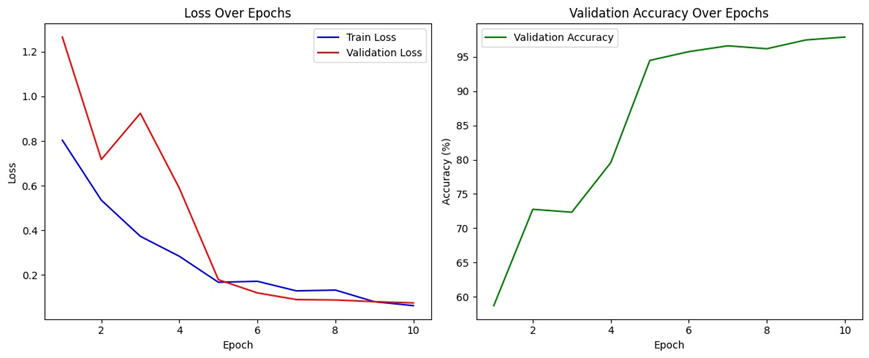
\includegraphics[keepaspectratio]{assets/loss-of-epochs-and-validation-accuracy.png}}

}

\caption{\label{fig-loss}Loss over Epochs and Validation Accuracy over
Epochs}

\end{figure}%

\begin{figure}

\centering{

\pandocbounded{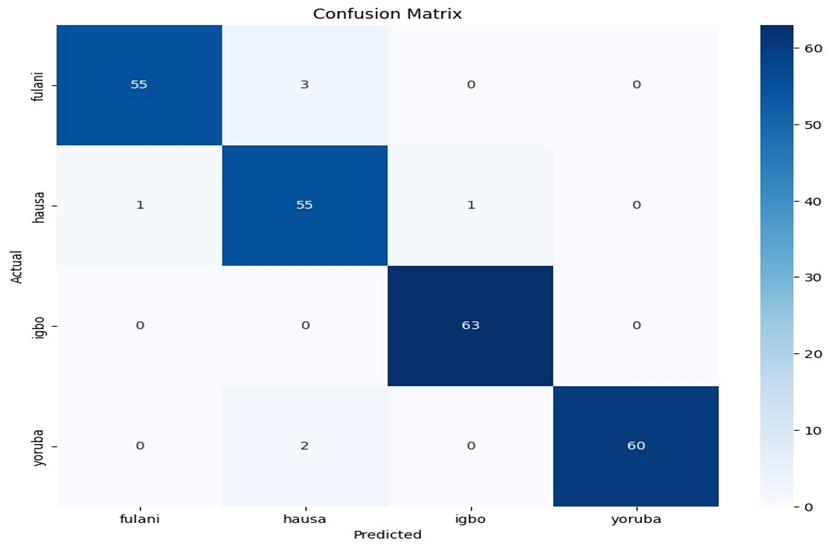
\includegraphics[keepaspectratio]{assets/confusion-matrix.png}}

}

\caption{\label{fig-confusion-matrix}Confusion matrix}

\end{figure}%

\subsection{Discussion}\label{discussion}

The superior performance of EfficientNet-B0 suggests its suitability for
image classification tasks involving cultural garments
\citeproc{ref-yuan_research_2025}{{[}10{]}}. The results affirm the
potential of deep learning models in automating the recognition of
traditional attires, which can be instrumental in cultural preservation
efforts.

\subsection{Conclusion}\label{conclusion}

This project successfully demonstrates the application of deep learning
techniques in classifying Nigerian traditional attire. The developed
models can serve as foundational tools for cultural education platforms,
virtual museums, and fashion industry applications. Future work may
involve expanding the dataset to include more ethnic groups and
exploring real-time classification systems.

\subsection*{Acknowledgment}\label{acknowledgment}
\addcontentsline{toc}{subsection}{Acknowledgment}

The authors wish to acknowledge the efforts of the entire team at Arewa
Data Science

\subsection*{References}\label{references}
\addcontentsline{toc}{subsection}{References}

\phantomsection\label{refs}
\begin{CSLReferences}{0}{0}
\bibitem[\citeproctext]{ref-ebby_traditional_2024}
\CSLLeftMargin{{[}1{]} }%
\CSLRightInline{Ebby, {``The {Traditional} {Attires} {Of} {Nigerian}
{Tribes},''} \emph{Inspiration with Lois{\textbar} Lifestyle {\textbar}
Nigeria}. Jun-2024 {[}Online{]}. Available:
\url{https://loispiration.com/2024/06/17/the-traditional-attires-of-nigerian-tribes/}.
{[}Accessed: 31-May-2025{]}}

\bibitem[\citeproctext]{ref-Ministry_of_Information_Culture_and_Tourism_2025}
\CSLLeftMargin{{[}2{]} }%
\CSLRightInline{Ministry of Information, Culture and Tourism, {``Culture
-- {MFA} {Press} {Center}.''} {[}Online{]}. Available:
\url{https://foreignaffairs.gov.ng/nigeria/nigeria-culture/}.
{[}Accessed: 31-May-2025{]}}

\bibitem[\citeproctext]{ref-he_deep_2016}
\CSLLeftMargin{{[}3{]} }%
\CSLRightInline{K. He, X. Zhang, S. Ren, and J. Sun, {``Deep {Residual}
{Learning} for {Image} {Recognition},''} in \emph{2016 {IEEE}
{Conference} on {Computer} {Vision} and {Pattern} {Recognition}
({CVPR})}, 2016, pp. 770--778 {[}Online{]}. Available:
\url{http://ieeexplore.ieee.org/document/7780459/}. {[}Accessed:
31-May-2025{]}}

\bibitem[\citeproctext]{ref-tan_efficientnet:_2019}
\CSLLeftMargin{{[}4{]} }%
\CSLRightInline{M. Tan and Q. V. Le, {``{EfficientNet}: {Rethinking}
{Model} {Scaling} for {Convolutional} {Neural} {Networks},''} 2019
{[}Online{]}. Available: \url{https://arxiv.org/abs/1905.11946}.
{[}Accessed: 31-May-2025{]}}

\bibitem[\citeproctext]{ref-alshagathrh_efficient_2023}
\CSLLeftMargin{{[}5{]} }%
\CSLRightInline{F. M. Alshagathrh, S. Musleh, M. Alzubaidi, J.
Schneider, and M. S. Househ, {``Efficient {Detection} of {Hepatic}
{Steatosis} in {Ultrasound} {Images} {Using} {Convolutional} {Neural}
{Networks}: {A} {Comparative} {Study},''} Oct. 2023 {[}Online{]}.
Available:
\url{https://manara.qnl.qa/articles/journal_contribution/Efficient_Detection_of_Hepatic_Steatosis_in_Ultrasound_Images_Using_Convolutional_Neural_Networks_A_Comparative_Study/26535460/1}.
{[}Accessed: 01-Jun-2025{]}}

\bibitem[\citeproctext]{ref-kansal_resnet-50_2024}
\CSLLeftMargin{{[}6{]} }%
\CSLRightInline{K. Kansal, T. B. Chandra, and A. Singh, {``{ResNet}-50
vs. {EfficientNet}-{B0}: {Multi}-{Centric} {Classification} of {Various}
{Lung} {Abnormalities} {Using} {Deep} {Learning},''} \emph{Procedia
Computer Science}, vol. 235, pp. 70--80, Jan. 2024 {[}Online{]}.
Available:
\url{https://www.sciencedirect.com/science/article/pii/S1877050924006768}.
{[}Accessed: 01-Jun-2025{]}}

\bibitem[\citeproctext]{ref-pamungkas_leaf_2023}
\CSLLeftMargin{{[}7{]} }%
\CSLRightInline{W. G. Pamungkas, M. I. P. Wardhana, Z. Sari, and Y.
Azhar, {``Leaf {Image} {Identification}: {CNN} with {EfficientNet}-{B0}
and {ResNet}-50 {Used} to {Classified} {Corn} {Disease},''} \emph{Jurnal
RESTI (Rekayasa Sistem dan Teknologi Informasi)}, vol. 7, no. 2, pp.
326--333, Mar. 2023 {[}Online{]}. Available:
\url{http://www.jurnal.iaii.or.id/index.php/RESTI/article/view/4736}.
{[}Accessed: 01-Jun-2025{]}}

\bibitem[\citeproctext]{ref-shams_skin_2025}
\CSLLeftMargin{{[}8{]} }%
\CSLRightInline{M. Y. Shams \emph{et al.}, {``Skin {Disease}
{Classification}: {A} {Comparison} of {ResNet50}, {MobileNet}, and
{Efficient}-{B0},''} \emph{Journal of Current Multidisciplinary
Research}, vol. 1, no. 1, pp. 1--7, Jan. 2025 {[}Online{]}. Available:
\url{https://jcmr.journals.ekb.eg/article_407474.html}. {[}Accessed:
01-Jun-2025{]}}

\bibitem[\citeproctext]{ref-li_cross-entropy_2024}
\CSLLeftMargin{{[}9{]} }%
\CSLRightInline{K. Li and F. Li, {``Cross-{Entropy} {Optimization} for
{Hyperparameter} {Optimization} in {Stochastic} {Gradient}-based
{Approaches} to {Train} {Deep} {Neural} {Networks},''} Sep. 2024
{[}Online{]}. Available: \url{http://arxiv.org/abs/2409.09240}.
{[}Accessed: 01-Jun-2025{]}}

\bibitem[\citeproctext]{ref-yuan_research_2025}
\CSLLeftMargin{{[}10{]} }%
\CSLRightInline{W. Yuan and Y. Ge, {``Research on national pattern
innovation fusion and packaging design system based on efficient net
image recognition and transfer learning algorithm,''} \emph{GeoJournal},
vol. 90, no. 2, p. 78, Apr. 2025 {[}Online{]}. Available:
\url{https://link.springer.com/10.1007/s10708-025-11325-5}. {[}Accessed:
01-Jun-2025{]}}

\end{CSLReferences}


% Can use something like this to put references on a page
% by themselves when using endfloat and the captionsoff option.
\ifCLASSOPTIONcaptionsoff
  \newpage
\fi

% trigger a \newpage just before the given reference
% number - used to balance the columns on the last page
% adjust value as needed - may need to be readjusted if
% the document is modified later
%\IEEEtriggeratref{8}
% The "triggered" command can be changed if desired:
%\IEEEtriggercmd{\enlargethispage{-5in}}

% Uncomment when use biblatex with style=ieee
%\renewcommand{\bibfont}{\footnotesize} % for IEEE bibfont size

\pagebreak[3]
% that's all folks
\end{document}

